\documentclass{article}
\usepackage{fancyhdr}
\usepackage{amsmath}
\usepackage{amsthm}
\usepackage{amssymb}
\usepackage{graphicx}
\usepackage{float}
\usepackage{subcaption}
\usepackage{hyperref}
\usepackage{listings}
\usepackage{color}
\usepackage{tikz}
\usepackage{pgfplots}
\usepackage{pgfplotstable}
\usepackage{listings}
\usepackage{color}
\usepackage{tikz}
\usepackage{amsthm}
\usepackage{soul}
\usepackage[margin=15mm]{geometry}

\definecolor{dkgreen}{rgb}{0,0.6,0}
\definecolor{gray}{rgb}{0.5,0.5,0.5}
\definecolor{mauve}{rgb}{0.58,0,0.82}
\hypersetup{colorlinks=true,linkcolor=blue, linktocpage}
% Set up fancy header
\pagestyle{fancy}
\fancyhf{} % Clear default header and footer
\rhead{Keith Wesa} % Right header
\lhead{MAT Written Assingment 3:} % Left header
\rfoot{Page \thepage} % Right footer

\author{Keith Wesa}
\title{MAT 215 - Written Homework 1}
\date{\today}

\begin{document}
\section*{Question 1}
\textbf{For each set $S$ given below, describe the set using other two notations: 
sentence notation, roster notation, or set-builder notation.} (Hint: to find a suitable sentence
for b. and c, think about what the set is describing. The set-builder form for a and b is not unique.)
(Note: When describing the set in roster notation, you need to provide enough elements to make 
the set in roster notation, you need to provide enough elements to make the set clear.) \textbf{[6 Marks]}
\subsection*{a. The set $S$ of integers divisible by 3 and 5.}
    
    \begin{itemize}
        \item[] \hl{\textbf{Roster Notation: } $S = \{15, 30 , 45, 60, 75, 90\}$}
        \item[] \hl{The mistake that I made was I forgot to include the negative numbers.}
        \item[] \textbf{Roster Notation: } $S = \{\pm 15, \pm 30, \pm 45,\pm 60,\pm 75,\pm 90\}$ --- This is the correct answer.
        \item[] \textbf{Set-Builder Notation: } $S = \{n \in \mathbb{Z} : n = 3k \land n = 5p\}$
        \begin{proof}
        \begin{center} 
        \begin{tabular}{|c|c|c|c|} 
        \hline $k$ & $p$ & $3k$ & $5p$ \\ 
        \hline 
        1 & 1 & 1 & 1 \\
        1 & 0 & 0 & 0  \\
        0 & 1 & 0 & 0 \\
        0 & 0 & 0 & 0  \\
\hline 
\end{tabular} 
\end{center}
        \item[] In order to satisfy the condition for $S$, $n$ must be a multiple of both 3 and 5. The statement would be false any other way.
        \end{proof}
\subsection*{b. $S =\{1,2,3,4,6,12\}$}  

    \item[] \textbf{Sentence Notation: } The set of all positive integers that are factors of 12.
    \item[] \textbf{Set-Builder Notation: } 
    \begin{align*}
        S &=\{1,2,3,4,6,12\} \\
        P &= \{12, 6, 4, 3, 2, 1\}\\ 
        S &= \{\forall n \in S(n) \forall p \in P(p) : n = \frac{12}{p} \} \\
    \end{align*}
    \begin{itemize}
        \item I thought this was an interesting question, and I couldn't figure out how to properly write out an answer for it
        what I find interesting is as the number $n$ increases then number for $p$ decreases. I'm not sure how to properly write this out in set-builder notation.
        So, I just started throwing math at it. 
    \end{itemize}
    \item[]
    \subsection*{c. $S = \{4^k : k \in \mathbb{Z}\}$}
    \item[] \textbf{Sentence Notation: } The set of integers that raise 4 to the power of $k$.
    \item[] \textbf{Set-Builder Notation: } $S = \{1, 4, 16, 64\}$
    \item[] \hl{The mistake that I made was I forgot to include the negative numbers for $k$.}
    \item[] \textbf{Set-Builder Notation: } $S = \{... ,\frac{1}{16},\frac{1}{4},1, 4, 16,...\}$
\end{itemize} 
\newpage
\section*{Question 2}
If you revisit our proof that $sqrt(2)$ is irrational, you will see that negation played an
important role. There are in fact two methods of proof for which negation is the
necessary first step: proof by contradiction and proof by contraposition (we will
explore these both later in the course). It is then important that we understand
how to find the negation of a statement.
\subsection*{a. Identify if each of the following sentences are statements. For each statement, write a negation.}
\subsubsection*{i. There exists a pair of irrational number $a$ and $b$ such that $a \times b$ is a rational number.}
\begin{itemize}
    \item[] \textbf{Statement: } True
    \begin{proof}
        Let $a = b$, $a = \sqrt{2}$, $b = \sqrt{2}$
           \begin{align*}
               a &= \sqrt{2} \\
               b &= \sqrt{2} \\
               a \times b &= \sqrt{2} \times \sqrt{2} \\
               a \times b &= 2 \\
           \end{align*}
   \end{proof}
    \item[] \textbf{Negation: } There does not exist a pair of irrational numbers $a$ and $b$ such that $a \times b$ is a rational number.
    \begin{proof}
        Let $a = b$, $a = \pi$, $b = \pi$
           \begin{align*}
               a &= \pi \\
               b &= \pi \\
               a \times b &= \pi \times \pi \\
               a \times b &= \pi^2 \\
           \end{align*}
    \end{proof}
    \item[] \hl{\textbf{What I forgot:} I forgot to include the negation}
    \item[] \textbf{Negation:} $a \times b$ is rational.
\end{itemize}

 \subsubsection*{ii. The set $\{3n: n \in \mathbb{N}\}$.}
\begin{itemize}
    \item[] \textbf{Statement: } True
    \begin{proof}
        Let $n = 1$, $n = 2$, $n = 3$
           \begin{align*}
               3 \times 1 &= 3 \\
               3 \times 2 &= 6 \\
               3 \times 3 &= 9 \\
           \end{align*}
    \end{proof}
    \item[] \textbf{Negation: } The set $\{3n: n \in \mathbb{N}\}^C$ 
    \begin{proof}
        Let $n = 1$, $n = 2$, $n = 3$
           \begin{align*}
               3 \times 1 &= 3 \\
               3 \times 2 &= 6 \\
               &\{3n: n \in \mathbb{N}\}^C \\ 
               &= (3 \cup 6 ) \\               
           \end{align*}
    \end{proof}
\end{itemize}
\subsubsection*{iii. The sum of interior angles of a triangle is 180 degrees.}
\begin{itemize}
    \item[] \textbf{Statement: } True
    \begin{proof}
        \begin{align*}
            \text{Let } a &= 60^\circ \\
            \text{Let } b &= 60^\circ \\
            \text{Let } c &= 60^\circ \\
            a + b + c &= 180^\circ \\
        \end{align*}
    \end{proof}
    \item[] \textbf{Negation: } The sum of interior angles of a triangle is not 180 degrees.
    \begin{proof}
        \begin{align*}
            a + b + c &\neq 180^\circ \\
        \end{align*}
    \end{proof}
\end{itemize}
\subsection*{b. Compose two mathematical statements (one quantified and on non-quantified), and 
two mathematical non-statements. For each statement, write a negation.}
\begin{itemize}
    \item[] \hl{\textbf{What I did wrong: I didn't even see this problem... Here's my answer.}}\
\end{itemize}
\subsubsection*{i. Mathematical Statement}
 \begin{itemize}
    \item[Statement 1]
    \begin{itemize}
     \item[] \textbf{Quantified Statement: } For all $n$ that is a positive integer, $n$ is divisible by 2.
     \item[] \textbf{Negation: } There exists a positive integer $n$ that is not divisible by 2.
     \end{itemize}
    \item[Statement 2]
    \begin{itemize}
     \item[] \textbf{Non-Quantified Statement: } If $n$ is greater than $m$ the statement is true.
     \item[] \textbf{Negation: } If $n$ is less than or equal to $m$ the statement is false.
    \end{itemize}
\end{itemize}
\subsubsection*{ii. Mathematical Non-Statement}
\begin{itemize}
    \item[Statement 1]
    \begin{itemize}
     \item[] \textbf{Quantified Non-Statement: } $f(0) = \frac{1}{x} = \text{undefined}$ 
     \item[] \textbf{Negation: } $f(0) = \frac{1}{x} \neq \text{undefined}$
    \end{itemize}
    \item[Statement 2]
    \item[] \textbf{Non-Quantified Non-Statement: } $x^2 + 2x + 1 = 0$
    \item[] \textbf{Negation: } $x^2 + 2x + 1 \neq 0$
    \end{itemize}
    \newpage
\section*{Question 3}

\begin{proof}
    \begin{itemize}
    Let’s consider two pairs of positive integers: (a, b) and (c, d), where a, b, c, d
are positive integers. We are given that the product of the first pair is larger than
the product of the second pair, i.e., $ab > cd$
\item[] Now, let's analyze the sum of each pair:
\item[] Sum of the first pair: $a + b$
\item[] Sum of the second pair: $c + d$
\item[] We want to prove that if $ab > cd$, then $a + b > c + d$. Let's assume, for the sake of contradiction, that $a + b \leq c + d$.
Now, we can rearrange this inequality to get:
\begin{align*}
    a &\leq c + d - b\\
\end{align*}
\item[] Now, multiply both sides by $b$ to get:
\begin{align*}
    ab &\leq bc + bd - b^2\\
\end{align*}
\item[] Since $ab > cd$ (as given in the problem), we have a contradiction because ab
cannot be both greater than and less than $b(c + d)$. Therefore, our assumption that
$a + b \leq c + d$ must be false. This implies that $a + b > c + d$. So, we have successfully
proven that if the product of one pair of positive integers is larger than the product
of another pair, then the sum is also larger.
\end{itemize}
\end{proof}
\begin{itemize}
    \item[a.] As we saw in Assignment 2 Question 1f., this statement is in fact false.
Critique the “proof” given by ChatGPT. (Hint: What statements in the
proof are correct? What statements in the proof are false? What statements
in the proof are out of place? What statements in the proof make no sense?)
    \begin{itemize}
        \item[1.] ChatGPT's proof was not a proof, it was a statement. In order to prove something you have to prove it against something else. 
        in the example given:
        \item[] \textbf{Example:} Define odd number as $n = 2p + 1$ for some integer $p$.
        \item[] \textbf{Explanation} This establishes a working definition. From here you can begin to proved something about $n$.
        \item[]
        \item[2.] There is an assumption that $a + b \leq c + d$ which is not true, because the domain of the problem is not defined.
        So, there is no telling if $a + b \leq c + d$ is true or not.
        \item[]
        \item[] \hl{\textbf{What I did Wrong: } This wasn't exactly what you were looking for.}
        \item[] \textbf{What you were looking for: } This proof aims for contradiction, and it fails to do so. 
    \end{itemize}
\item[b.] Prompt ChatGPT to prove that $\sqrt{2}$ is irrational. How does the proof compare 
to our proof during class? 
\begin{itemize}
    \item[] \textbf{ChatGPT:} Prove that $\sqrt{2}$ is irrational.
\begin{figure}[H]
    \centering
    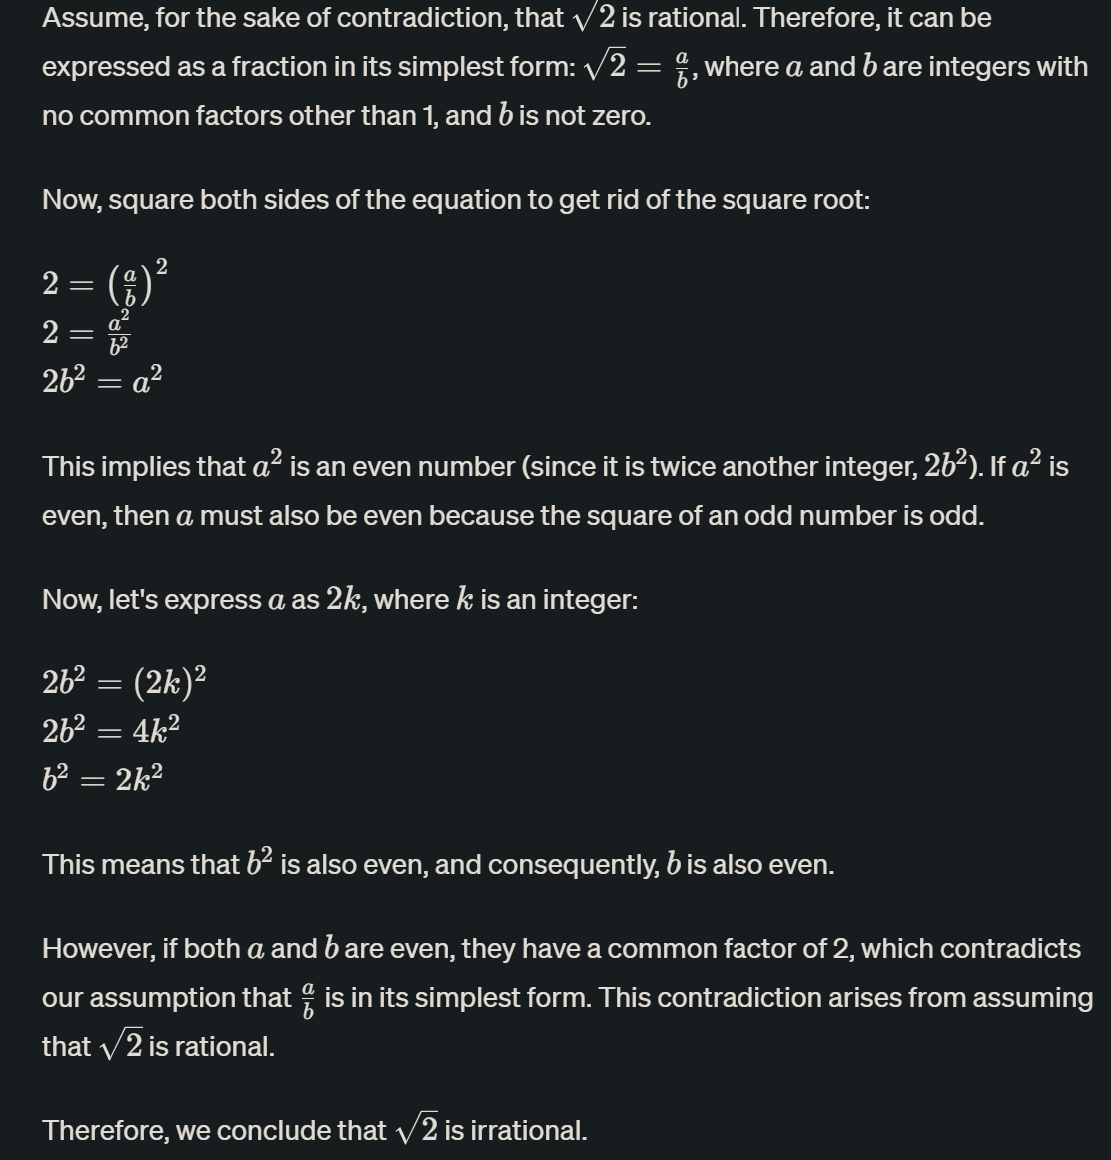
\includegraphics[width=0.5\textwidth]{ChatGPTsqrt2.png}
    \caption{ChatGPT Proof of $\sqrt{2}$ is irrational.}
    \label{fig:example}
\end{figure}
\item[]
\item[] \textbf{Answer:} It differs slightly, but for the most part it is the same. We chose different variables such as $p$ and $q$ instead of $a$ and $b$.
\item[]
\end{itemize}
    \item[c.] Why do you think ChatGPT was able to provide a correct proof of that $\sqrt{2}$ is irrational, but failed in the above example?
    \begin{itemize}
        \item[] I think that ChatGPT gave a correct proof for the irrationality of $\sqrt{2}$ is because ChatGPT is a predictive text modeler not a logic machine. 
        Odds are that there is more information about the proof of $\sqrt{2}$ being irrational then the example in the above example. 
        \item[] The GPT in ChatGPT stands for Generative Pre-trained Transformer. The way it works is, that we give the machine a prompt and it takes publicly available information 
         or whatever is in its data-set and gives you a response based on what would statistically make sense given its parameters. 
        \end{itemize}
        \newpage
    \item[d.] In what ways do you think ChatGPT can be a useful tool regarding proofs in mathematics? 
        \begin{itemize}
            \item[] My answer is that ChatGPT isn't built for doing mathematical proofs outside of its data-sets. There are certain areas of math where it works well such as propositional logic, but for the most part its unreliable.
         That being said, it doesn't mean that there won't exist a machine that can be designed to prove something. In fact there have been many built specifically for that purpose, 
         I'd encourage you to read \href{https://www.popularmechanics.com/science/math/a33820013/keller-conjecture-old-math-problem-solved/}{Problem solved: 90-year-old math problem cracked by AI} 
        they built a machine designed specifically to prove a conjecture. All that being said, my personal opinion is relying on a AI to me is like relying on a GPS system to get you around everywhere.
         it's handy but if you don't know how to read a map or understand directions do you really know where you're going?
        \end{itemize}
 \end{itemize}

\end{document}
